\documentclass[11pt]{article}
\usepackage[T1]{fontenc}
\usepackage{lmodern}
\usepackage{amsmath,amssymb}
\usepackage{booktabs,array,float}
\usepackage{tikz}
\usetikzlibrary{arrows.meta,positioning}
\usepackage{listings}
\usepackage{xcolor}
\usepackage{enumitem}
\usepackage[font=small]{caption}
\usepackage[hidelinks]{hyperref}

\captionsetup[table]{position=below,skip=6pt}
\newcolumntype{C}[1]{>{\centering\arraybackslash}p{#1}}
\lstset{basicstyle=\ttfamily\footnotesize,columns=fullflexible,keepspaces=true,
  breaklines=true,frame=single,rulecolor=\color{black!25},backgroundcolor=\color{black!3},
  xleftmargin=2pt,xrightmargin=2pt,aboveskip=6pt,belowskip=6pt}
\newcommand{\cmd}[1]{\texttt{#1}}
\setlist{itemsep=2pt,topsep=4pt}
\setlength{\emergencystretch}{3em}

\title{Camera to \LaTeX: Instructions\\[2pt]\large Version 1 for the EE\,105 board}
\author{Project team}
\date{November 17, 2026 \textperiodcentered{} hard deadline December 1}

\begin{document}
\maketitle

\section{What you are building}

The board takes a grayscale photo of one printed line and sends it to the laptop over USB. The
laptop splits the photo into symbols, recognizes each symbol with a small neural network, works
out how the symbols sit relative to each other (superscripts, subscripts, fractions), and writes
the line as \LaTeX. Each line you accept is added to a document that \cmd{pdflatex} turns into a
PDF. The board does no recognition: it runs one short sketch, \cmd{firmware/capture/capture.ino},
that answers ``send me a frame''. Everything else is Python in this repository, and every number
you may need to tune lives in \cmd{config.py}.

\begin{figure}[H]
\centering
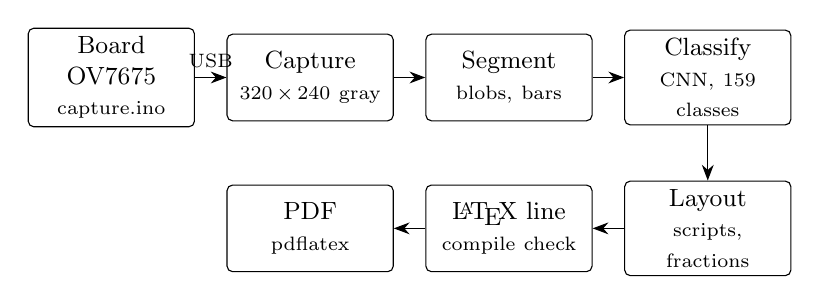
\begin{tikzpicture}[node distance=4mm, every node/.style={font=\small},
  box/.style={draw, rounded corners=2pt, align=center, minimum height=11mm, inner sep=3pt, text width=19mm},
  >={Stealth[length=2mm]}]
\node[box] (b) {Board\\OV7675\\\scriptsize capture.ino};
\node[box, right=of b] (c) {Capture\\\scriptsize 320\,$\times$\,240 gray};
\node[box, right=of c] (s) {Segment\\\scriptsize blobs, bars};
\node[box, right=of s] (k) {Classify\\\scriptsize CNN, 159 classes};
\node[box, below=7mm of k] (l) {Layout\\\scriptsize scripts, fractions};
\node[box, left=of l] (t) {\LaTeX{} line\\\scriptsize compile check};
\node[box, left=of t] (p) {PDF\\\scriptsize pdflatex};
\draw[->] (b) -- node[above, font=\scriptsize]{USB} (c);
\draw[->] (c) -- (s);
\draw[->] (s) -- (k);
\draw[->] (k) -- (l);
\draw[->] (l) -- (t);
\draw[->] (t) -- (p);
\end{tikzpicture}
\caption{The pipeline. Only the first box runs on the board; the rest runs on the laptop.}
\end{figure}

A frame is 320 by 240 pixels at one byte per pixel, so 76{,}800 bytes cross the cable per photo.
The classifier knows 159 classes made of 182 symbols: every visible ASCII character plus the common
math symbols (Greek letters, operators, relations, arrows, set symbols, $\sum$, $\int$, $\sqrt{\ }$,
$\mathbb{R}$ and friends). Symbols that print almost identically share a class (o, O and 0; l, I
and $|$; c and C; the period and $\cdot$; the hyphen and the underscore), and the layout stage
decides which one it was from its size, height on the line and neighbours. The full list is
\cmd{symbols.csv}.

\section{What you need}

\begin{table}[H]
\centering
\begin{tabular}{C{3.0cm}C{8.6cm}}
\toprule
\textbf{Item} & \textbf{Details} \\
\midrule
Board & EE\,105 carrier, Arduino Nano 33 BLE Sense Lite, OV7675 camera \\
Cable & USB data cable (a charge-only cable shows no port) \\
Laptop & Python 3.10 to 3.13 (TensorFlow has no wheels for newer versions yet) \\
\TeX{} & TeX Live, MacTeX or MiKTeX, with \cmd{pdflatex} on the path \\
Arduino IDE & version 2, board package ``Arduino Mbed OS Nano Boards'' \\
Rig & a stand that holds the board face down about 15\,cm above the page, and a desk lamp \\
Printer & anything; print at 100\,\% (``actual size'') \\
\bottomrule
\end{tabular}
\caption{Parts and software.}
\end{table}

\section{Set up the laptop}

\begin{lstlisting}
cd camera-to-latex
python3.12 -m venv .venv
source .venv/bin/activate       # Windows: .venv\Scripts\activate
pip install -r requirements.txt
python -m pytest -q             # 45 tests; none need the board
python -m pipeline.main --pdf   # warns if pdflatex is missing
\end{lstlisting}

If TensorFlow will not install, everything still works with the fallback classifier
(\cmd{--backend sklearn} in Section~\ref{sec:train}); it is weaker, so keep trying to get the
convolutional network for the final demo.

\section{Flash the board}

\begin{enumerate}
\item In the Arduino IDE, install the board package \emph{Arduino Mbed OS Nano Boards} and select
  the board \emph{Arduino Nano 33 BLE}.
\item Install the camera library \emph{Arduino\_OV767X}. If your digit-recognition sketch used the
  copy inside \emph{Harvard\_TinyMLx}, keep that one instead; do not install both.
\item Open \cmd{firmware/capture/capture.ino}, choose the port and press Upload. If the upload
  fails, double-tap the reset button (the orange LED pulses) and upload again.
\item Close the Serial Monitor: Python cannot open the port while it is open.
\end{enumerate}

The four settings at the top of the sketch are for bring-up only.

\begin{table}[H]
\centering
\begin{tabular}{C{3cm}C{1.5cm}C{6.8cm}}
\toprule
\textbf{Setting} & \textbf{Default} & \textbf{Change it when} \\
\midrule
\cmd{USE\_GRAYSCALE} & 1 & frames look wrong in GRAYSCALE mode: set 0 to use YUV422 and keep the brightness bytes \\
\cmd{Y\_OFFSET} & 0 & with YUV422 the picture looks like noise or a negative: set 1 \\
\cmd{TEST\_PATTERN} & 0 & set 1 to receive the camera's colour bars (vertical gray bands) instead of the scene \\
\cmd{CAMERA\_FPS} & 1 & the soak test passes at 1 and you want a smoother preview: try 5 \\
\bottomrule
\end{tabular}
\caption{Sketch settings.}
\end{table}

\section{First light}

\begin{lstlisting}
python -m pipeline.capture --list       # ports (or set SERIAL_PORT in config.py)
python -m pipeline.capture --ping       # board answers: 320x240, 1 byte per pixel
python -m pipeline.capture --grab first.png
python -m pipeline.capture --soak 100   # gate G1: 100/100 frames OK
\end{lstlisting}

Open \cmd{first.png}. If it is upside down or mirrored, set \cmd{FLIP\_H}, \cmd{FLIP\_V} or
\cmd{ROTATE\_DEG} in \cmd{config.py} until the preview in \cmd{python -m pipeline.main} reads
normally. Saved photos are always the raw frames; the flips are applied when they are read, so
changing them later never spoils data you already took.

\section{Build the rig and check the size}
\label{sec:rig}

Hold the board face down over the page, light the page from the side at about 45 degrees (no
glare, no shadow of the board), and keep the page flat. What matters is how many pixels a capital
letter covers. With the camera at height $d$ above the page and a horizontal field of view
$\theta$, the strip of page in view is
\[
  w = 2\,d\,\tan\frac{\theta}{2}.
\]
At $d = 15$\,cm this is about 13.3 to 15.0\,cm across 320 pixels, so 21 to 24 pixels per
centimetre, and a 40\,pt capital (0.96\,cm) covers about 20 to 23 pixels. Measure it: photograph
a test line, zoom in, and count the pixels from the bottom to the top of a capital.

On fake photos of the 60 test lines, the share of lines read exactly went from 62\,\% at
20\,px capitals to 70\,\% at 24\,px and 80\,\% at 30\,px (fallback model, synthetic training data
only). Thin strokes of the Computer Modern font break apart and neighbouring letters touch when
capitals are small. So if you measure fewer than about 26 pixels, lower the board to about
12.5\,cm (the widest test line is 9.7\,cm at 40\,pt and still fits in the 11 to 12.5\,cm view)
or print at 48\,pt, and check that the picture is still sharp at the new height.

\section{Print the materials}

Both are already generated in the repository; regenerate them only if you change
\cmd{symbols.csv} or the test lines.

\begin{lstlisting}
python -m tools.make_sheets                     # sheets/sheets.pdf, 9 pages
python -m tools.make_test_lines --pdf --names   # test_set/test_lines.pdf, 16 pages
\end{lstlisting}

Print at 100\,\% and check with a ruler that the corner squares on the sheets are 5\,mm wide.
Each sheet block has 7 by 5 cells; the hollow corner square marks the top left, so a page that
is turned around still crops correctly. The 182 symbols fill six blocks, and the spare cells
repeat symbols that are easy to confuse. The three sets differ: set A prints letters upright as in
text, set B italic as in formulas, and set C mixes both. Math lines on the test sheet are printed
in display style, which makes fractions larger and leaves more room around their bars.

\section{Collect real data}
\label{sec:data}

\paragraph{Sheets (gate G1).} Photograph every block three times, moving the page about a
centimetre and changing the light between shots:
\begin{lstlisting}
python -m pipeline.capture --series data/sheets --names-file sheets/photo_names.txt
python -m tools.crop_sheet --debug
\end{lstlisting}
In the capture window, SPACE saves the next name (\cmd{A1\_1}, \cmd{A1\_2}, \ldots), \cmd{b} goes
back and \cmd{n} skips. All four corner squares must be in view. The cropper prints how many crops
each photo gave and lists photos to retake; open \cmd{data/sheets/debug/} and check that the grid
lines fall between the symbols. 54 photos give about 9 real crops per symbol, saved under
\cmd{data/crops\_real/<class>/}.

\paragraph{Test lines.} Photograph all 80 lines the same way:
\begin{lstlisting}
python -m pipeline.capture --series test_set/images --names-file test_set/photo_names.txt
\end{lstlisting}
Keep the line in the middle of the frame. Use the 20 dev lines (D01 to D20) for tuning and the 60
test lines (T01 to T60) only for reporting results, otherwise the numbers flatter the system.

\section{Train the classifier}
\label{sec:train}

\begin{lstlisting}
python -m model.make_synthetic   # about 65,000 crops, 1-2 minutes
python -m model.train            # the CNN (TensorFlow)
python -m model.evaluate         # held-out real crops: accuracy, confusions
\end{lstlisting}

\cmd{make\_synthetic} draws every symbol in every font it finds (Latin Modern and \TeX{} Gyre from
your \TeX{} installation, DejaVu and STIX from matplotlib, system fonts, and any font you put in
\cmd{data/fonts/}), then passes each drawing through a fake camera: random size, slight rotation,
thicker or thinner strokes, uneven light, blur and noise. Look at
\cmd{data/synthetic/preview\_*.png}: every row should show recognizable copies of its class. The
script also lists symbols that often break into pieces after thresholding, which is where
segmentation will struggle.

\cmd{train} mixes the synthetic crops with your real crops (repeated five times because there are
few of them), holds out the real crops of one photo in five, and reports accuracy on them. Gate G2
asks for at least 95\,\% there. The network has about 149{,}000 weights: two blocks of two
convolutions with pooling, a $1\times1$ convolution, a $4\times4$ grid kept to the end so the
position of strokes still counts, and a softmax over the 159 classes. If TensorFlow is not
available, \cmd{python -m model.train --backend sklearn} trains a multilayer perceptron on
stroke-direction (HOG) features in about a minute; it reached 97\,\% on held-out synthetic crops
here, but expect less on real ones.

If \cmd{evaluate} shows two classes being confused, photograph those sheet cells again under
different light and retrain. Public datasets can add variety (Appendix~\ref{app:data}), but your
own crops matter most because they come from the same camera.

\section{Run the app}

\begin{lstlisting}
python -m pipeline.main          # live, with the board
python -m pipeline.main --new    # new document (the old session is kept)
python -m pipeline.main --image photo.png --accept --pdf   # no board
\end{lstlisting}

\begin{table}[H]
\centering
\begin{tabular}{C{2.6cm}C{8.8cm}}
\toprule
\textbf{Key} & \textbf{Action} \\
\midrule
SPACE & read the line in view; boxes appear (green sure, red worth checking, blue fraction bar) \\
\cmd{a} or ENTER & accept the line (it is compile-checked first) \\
\cmd{e} & edit the \LaTeX{} in the terminal, then accept \\
\cmd{r} & reject and go back to the live view \\
\cmd{m} & mode: auto, text, math (math lines go in \verb|\[ \]|, text lines are paragraphs) \\
\cmd{u} & remove the last accepted line \\
\cmd{p} & build and open \cmd{out/document.pdf} \\
\cmd{s} & save the current frame to \cmd{data/raw/} \\
\cmd{q} or ESC & quit (the PDF is rebuilt if you accepted anything) \\
\bottomrule
\end{tabular}
\caption{Keys in the app window (click the window first).}
\end{table}

Accepted lines live in \cmd{out/session.json}, so a crash loses nothing and the PDF can be rebuilt
with \cmd{python -m pipeline.main --pdf}. The document preamble is \cmd{template/document.tex}.

\section{Measure and tune}

\begin{lstlisting}
python -m tools.eval_pipeline --split dev    # while tuning
python -m tools.eval_pipeline                # test lines, for the report
python -m tools.make_test_lines --render     # fake photos (no board needed)
python -m tools.eval_pipeline --images test_set/synthetic --split all
\end{lstlisting}

For each category (plain, scripts, fractions, mixed) the script reports the share of lines read
exactly, the token error rate, the share of predicted lines that compile, and the time per line.
Before comparing, both strings are normalized, so spacing, optional braces and synonyms such as
\verb|\le| and \verb|\leq| do not count as errors. The token error rate is the edit distance
between the predicted and expected token lists divided by the expected length,
\[
  \mathrm{TER} = \frac{d(\text{predicted}, \text{expected})}{|\text{expected}|},
\]
so one wrong token in a 20-token line is 5\,\%. Every line is written to
\cmd{results/eval\_*.csv}; read the failures before changing anything.

\begin{table}[H]
\centering
\begin{tabular}{C{3.4cm}C{1.6cm}C{6.2cm}}
\toprule
\textbf{Setting} & \textbf{Default} & \textbf{Effect} \\
\midrule
\cmd{THRESH\_C} & 10 levels & higher: less paper texture counted as ink, more broken strokes \\
\cmd{THRESH\_WEAK\_C} & 5 levels & lower: faint strokes rejoin their letter; \cmd{None} switches it off \\
\cmd{THRESH\_BLOCK} & 31\,px & about one symbol's size; larger copes worse with shadows \\
\cmd{MIN\_BLOB\_AREA} & 4\,px & smallest ink kept (a period is about 10\,px) \\
\cmd{MERGE\_MAX\_HEIGHT} & 1.5 caps & tallest symbol that pieces may be joined into ($j$ is 1.3) \\
\cmd{FRACTION\_MAX\_GAP} & 1.0 caps & farthest a numerator may sit from its bar \\
\cmd{CONF\_MIN} & 0.6 & below this the symbol is shown in red and may be repaired \\
\cmd{SPACE\_GAP} & 0.4 caps & wider gaps become spaces in text lines \\
\cmd{SCRIPT\_PENALTY} & 1.0 & higher: fewer symbols read as scripts \\
\cmd{LAYOUT\_LEVEL} & 3 & 1 plain lines only, 2 adds scripts, 3 adds fractions and roots \\
\bottomrule
\end{tabular}
\caption{Settings in \cmd{config.py} most worth tuning (a ``cap'' is the line's capital height).}
\end{table}

Change one setting at a time, rerun the dev lines, and keep the change only if the exact-line
rate goes up. If fractions cannot reach their target by gate G4 (November 25), set
\cmd{LAYOUT\_LEVEL = 2} and hand in plain and script lines.

\section{Troubleshooting}

\begin{table}[H]
\centering
\begin{tabular}{C{3.4cm}C{8.0cm}}
\toprule
\textbf{Symptom} & \textbf{What to do} \\
\midrule
No port listed & use a data cable; on Windows install the Arduino Mbed driver from the IDE \\
``port busy'' & close the Serial Monitor and any other Python window using the board \\
``ERR camera'' & reseat the camera, check the library choice (Section 4), power-cycle \\
Timeouts in the soak test & set \cmd{CAMERA\_FPS 1}, use a shorter cable, avoid USB hubs \\
Picture is noise & set \cmd{USE\_GRAYSCALE 0}, then try \cmd{Y\_OFFSET} 0 and 1 \\
Letters split into pieces & more light, larger capitals (Section~\ref{sec:rig}), lower \cmd{THRESH\_WEAK\_C} \\
Neighbouring letters merge & sharper focus, raise \cmd{THRESH\_C}, larger capitals \\
A second line is read & centre the wanted line; keep 4\,cm between printed lines \\
Fraction read as scripts & print in display style; check that the bar is unbroken in the photo \\
Line will not compile & press \cmd{e} and fix it; the error is printed in the terminal \\
Model and table differ & you edited \cmd{symbols.csv}: rerun \cmd{make\_synthetic} and \cmd{train} \\
\bottomrule
\end{tabular}
\caption{Common problems.}
\end{table}

\section{Schedule}

\begin{table}[H]
\centering
\begin{tabular}{C{1.2cm}C{2.4cm}C{7.4cm}}
\toprule
\textbf{Gate} & \textbf{Date} & \textbf{Check} \\
\midrule
G0 & Tue Nov 17 & laptops set up, tests pass, board flashed, sheets and test lines printed \\
G1 & Wed Nov 18 & soak test 100/100; 54 sheet photos cropped; 80 test lines photographed \\
G2 & Fri Nov 20 & plain lines go photo to PDF; at least 95\,\% on held-out real crops \\
G3 & Mon Nov 23 & script lines meet their target; README done; demo video recorded \\
G4 & Wed Nov 25 & fraction lines meet their target, or \cmd{LAYOUT\_LEVEL = 2} \\
G5 & Tue Dec 1 & hand-in: rehearsed twice on Nov 30, repository tagged \cmd{v1.0} \\
\bottomrule
\end{tabular}
\caption{Gates from the bring-up plan. Thanksgiving week (Nov 26 to 29) has nothing critical.}
\end{table}

\section{Where things are}

\begin{table}[H]
\centering
\begin{tabular}{C{3.6cm}C{7.8cm}}
\toprule
\textbf{Path} & \textbf{Contents} \\
\midrule
\cmd{config.py} & every tunable number \\
\cmd{symbols.csv} & classes, members, heights, \LaTeX{} and how to draw each symbol \\
\cmd{firmware/capture/} & the Arduino sketch \\
\cmd{pipeline/} & capture, segment, classify, layout, document, app \\
\cmd{model/} & synthetic data, training, evaluation, optional on-board export \\
\cmd{tools/} & sheets, sheet cropping, test lines, evaluation, datasets \\
\cmd{sheets/}, \cmd{test\_set/} & printable PDFs, layouts, line list, your photos \\
\cmd{data/}, \cmd{models/}, \cmd{out/}, \cmd{results/} & generated; not in git \\
\bottomrule
\end{tabular}
\caption{Repository map.}
\end{table}

\appendix

\section{Serial protocol}

The laptop sends one byte and the board answers. \cmd{p} returns the text line
\cmd{OK 320 240 1}. \cmd{c} returns one frame: the bytes \cmd{FRM1}, then width and height as
16-bit numbers, the bytes per pixel (always 1), the pixel count as a 32-bit number, the pixels row
by row, and a 16-bit checksum equal to the sum of the pixel bytes modulo 65{,}536. All numbers are
little-endian. The reader skips anything before \cmd{FRM1}, reports any line starting with
\cmd{ERR}, and retries a frame up to three times if the checksum or the timing fails.

\section{Datasets}
\label{app:data}

Version 1 is trained on synthetic crops and your own sheet crops. The public datasets below are
optional extras. The download script lists them and fetches the ones with a direct link (the
Kaggle ones need the Kaggle command-line tool and an account), and the import script converts the
first four into crops with the right relative size:
\begin{lstlisting}
python -m tools.download_datasets --list
python -m tools.download_datasets chars74k_fnt hasy
python -m tools.import_datasets chars74k_fnt hasy
python -m model.train --external
\end{lstlisting}
Check each licence on its page before use and cite what you use.

\begin{table}[H]
\centering
\begin{tabular}{C{2.6cm}C{6.2cm}C{2.4cm}}
\toprule
\textbf{Dataset} & \textbf{Contents} & \textbf{Use} \\
\midrule
Chars74K (Fnt) & digits and letters drawn from computer fonts & v1, recommended \\
TMNIST (94 chars) & every printable ASCII glyph in Google Fonts, 28\,$\times$\,28\,px & v1, recommended \\
HASYv2 & 168{,}233 handwritten symbols in 369 \LaTeX{} classes, 32\,$\times$\,32\,px & v1, small share \\
Kaggle math symbols & handwritten math symbols, 45\,$\times$\,45\,px & v1, small share \\
IM2LATEX-100K & 103{,}556 rendered formulas with their \LaTeX{} & revision 2 \\
MathWriting & 230{,}000 handwritten and 400{,}000 synthetic expressions & revision 2 \\
CROHME 2023 & handwritten expressions, competition data & revision 2 \\
\bottomrule
\end{tabular}
\caption{Public datasets and where they fit.}
\end{table}

The first two are printed text, like our input, so they help most. The handwritten ones add
variety but differ from print, so \cmd{model.train --external} limits external crops to a quarter
of the training set. The last three hold whole expressions rather than single symbols; they are for
the revision-2 idea of reading a whole line with one image-to-\LaTeX{} model.

\end{document}
